% SOURCE: hand-authored schematic; no experimental data.
\documentclass[tikz,border=4pt]{standalone}
\usepackage[T1]{fontenc}
\usepackage{lmodern}
\usepackage{amsmath}
\usetikzlibrary{arrows.meta,positioning,fit,backgrounds,shapes.geometric}
\definecolor{ink}{HTML}{243447}
\definecolor{blue}{HTML}{0072B2}
\definecolor{orange}{HTML}{D55E00}
\definecolor{muted}{HTML}{6B7280}
\definecolor{pale}{HTML}{EEF4F8}
\tikzset{
  box/.style={draw=ink,rounded corners=2pt,fill=pale,minimum width=2.35cm,
    minimum height=0.78cm,text width=2.15cm,align=center,
    font=\sffamily\small,inner xsep=2mm,inner ysep=1.5mm},
  arrow/.style={-{Latex[length=2mm]},line width=.65pt,draw=ink},
  note/.style={font=\sffamily\scriptsize\color{muted},align=center,
    text width=2.6cm,inner sep=1pt},
  fence/.style={draw=muted,dashed,rounded corners=3pt,inner sep=6pt}
}
\begin{document}
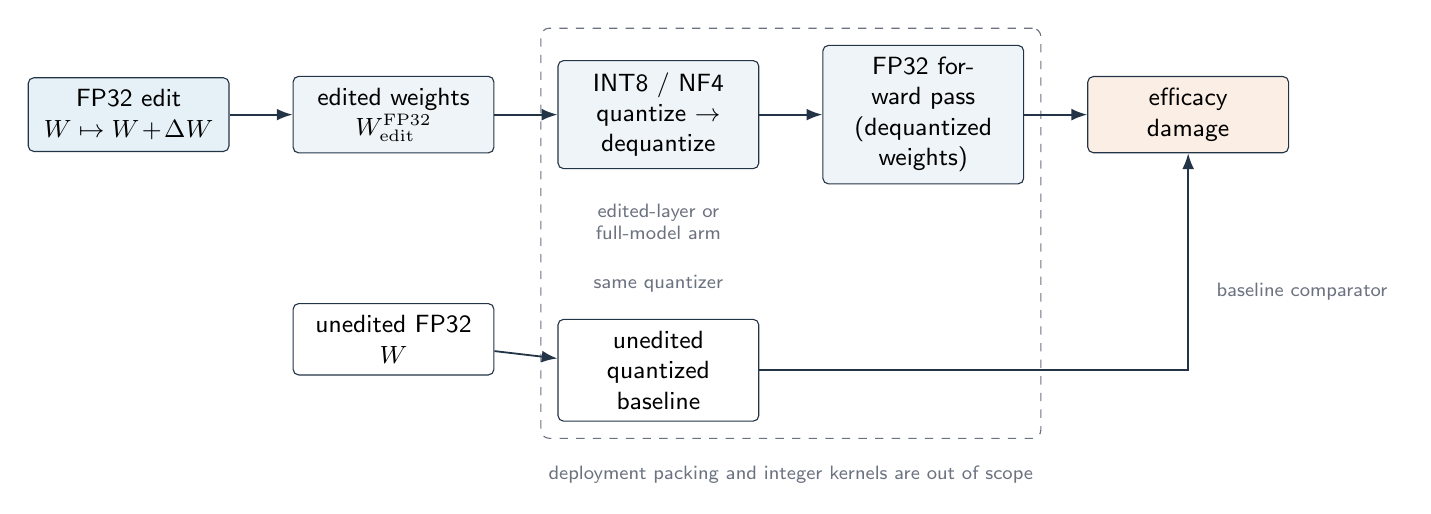
\begin{tikzpicture}[node distance=8mm and 8mm]
\node[box,fill=blue!10] (edit) {FP32 edit\\$W\mapsto W+\Delta W$};
\node[box,right=of edit] (weights) {edited weights\\$W_{\rm edit}^{\rm FP32}$};
\node[box,right=of weights] (qd) {INT8 / NF4\\quantize $\to$ dequantize};
\node[box,right=of qd] (refwd) {FP32 forward pass\\(dequantized weights)};
\node[box,fill=orange!10,right=of refwd] (out) {efficacy\\damage};
\draw[arrow] (edit)--(weights);
\draw[arrow] (weights)--(qd);
\draw[arrow] (qd)--(refwd);
\draw[arrow] (refwd)--(out);

\node[note,below=4mm of qd] (armnote) {edited-layer or\\full-model arm};
\node[box,below=19mm of weights,fill=white] (base) {unedited FP32\\$W$};
\node[box,below=19mm of qd,fill=white] (baseq) {unedited quantized\\baseline};
\node[note,above=3mm of baseq,text width=2.2cm] (sameq) {same quantizer};
\draw[arrow] (base)--(baseq);
\draw[arrow] (baseq.east) -| node[note,pos=.68,right=1.5mm,text width=2.5cm]
  {baseline comparator} (out.south);

\begin{scope}[on background layer]
\node[fence,fit=(qd)(refwd)(baseq)] (scope) {};
\end{scope}
\node[note,below=3mm of scope.south,text width=6.4cm]
  {deployment packing and integer kernels are out of scope};
\end{tikzpicture}
\end{document}
